% 必要な項目ができた場合は適宜サブセクションを追加してください

%\include{begin}
\section{入所式・教員紹介}

\subsection{日時・場所}
\begin{tabular}{p{2zw}rp{38zw}}
  日時 & : & 2019年4月5日(金) 15:30$\sim$16:10\\
  場所 & : & 大研修室
\end{tabular}

\subsection{目的}
施設の円滑な利用と利用規約について理解を促す.また,新入生に今後お世話になる教職員の方々を覚えてもらうきっかけを作る.

\subsection{タイムスケジュール}
\begin{longtable}{p{3zw}p{39zw}}
  15:30 & \textbf{◎ 入所式開始} \\
  %小野
        & \ \ \textbullet \ \ 司会者(立岩)の簡単な挨拶と,代表(宮尾)の紹介をする \\
        & \ \ \textbullet \ \ 代表による施設職員と新入生に向けた挨拶をする \\\\

  15:35 & \textbf{◎ 教員紹介開始} \\
        & \ \ \textbullet \ \ 司会者は,教員紹介の説明をする \\
        & \ \ \textbullet \ \ 司会者は教職員にマイクをリレー形式で渡していただくよう伝える \\
        & \ \ \textbullet \ \ 司会者は最初の教職員にマイクを渡し,並んでいる新入生の後ろ側を通り,スタッフの待機場所に移動する  \\
        & \ \ \textbullet \ \ 司会者は最後の教職員の近くで待機する \\
        & \ \ \textbullet \ \ 教職員に自己紹介を行ってもらう(1分/人) \\
        & \ \ \textbullet \ \ 教職員の自己紹介が終わり次第,司会者は最後の教職員からマイクをもらう \\
        & \ \ \textbullet \ \ 司会は教員紹介に参加できない先生と遅刻する先生の紹介を始める \\\\

  16:00 & \textbf{◎ 教員紹介終了} \\ %教員紹介が押すと推定
        & \ \ \textbullet \ \ 司会者は各スタッフを野外炊事の担当の班の出口側に並ぶように伝える \\
        & \ \ \textbullet \ \ この時待機していたスタッフは担当の班の先頭に並ぶ \\
        & \ \ \textbullet \ \ 司会者はスタッフに座るよう指示する \\\\

  16:05 & \textbf{◎ 施設職員さんによる施設説明} \\
        & \ \ \textbullet \ \ 司会者は施設職員さんによる施設利用の注意について説明があることを伝える \\
        & \ \ \textbullet \ \ 司会者は施設職員さんに説明をしていたいだくよう伝える \\
        & \ \ \textbullet \ \ 施設職員さんが施設利用の説明をする \\\\

  16:10 & \textbf{◎ 移動開始} \\
        & \ \ \textbullet \ \ 司会者は各班につく先生の名前をアナウンスするとともに,2班ずつ大研修室から野外炊事場に移動するように伝える \\
        & \ \ \textbullet \ \ 各班のスタッフは,担当の班を野外炊事場へと誘導する \\
        %& \ \ \textbullet \ \ この時,靴を入れていた袋は出口付近にいる袋回収係(?長通,生野,藤田(竜世))に渡す\\
        & \ \ \textbullet \ \ 全班退出後,片付け係(斎藤,堀川,高橋(慎))と鍵係(小谷)は大研修室の椅子は第一研修室へ,各班のプラカードは第四研修室へ運ぶ\\
        %& \ \ \textbullet \ \ 鍵係(岡本)は第二集会室の開錠を行う\\
        & \ \ \textbullet \ \ 全班退出後,司会者は野外炊事場へ移動する\\
        %& \ \ \textbullet \ \ ?岡本は運び終わったら第二集会室の鍵を閉める\\
        & \ \ \textbullet \ \ 片付け係(斎藤,堀川,高橋(慎))は片付けが終わったら野外炊事場の担当の班の場所へ移動する \\
        & \ \ \textbullet \ \ 小谷は宮尾からワゴン車到着の連絡があるまで,第一研修室前で待機する \\
        & \ \ \textbullet \ \ 移動時点でワゴン車が到着していて,誘導の必要がない場合は,事務室に研修室の施錠をお願いし,片付け係とともに野外炊事場へ向かう \\

        & \textbf{※ ワゴン車到着} \\
        & \ \ \textbullet \ \ ワゴン車が到着したら入交さんに宮尾へ連絡してもらう \\
        & \ \ \textbullet \ \ 宮尾は連絡が来次第,小谷へ連絡をする \\
        & \ \ \textbullet \ \ 小谷は連絡が来たら遅れてきた新入生と事務員さんを迎えに行く \\
        & \ \ \textbullet \ \ 小谷は事務室にお願いして第一・二研修室の鍵を開けてもらい,新入生と事務員さんの荷物を置く \\
        & \ \ \textbullet \ \ 置いたら事務室で施錠してもらい,野外炊事場へ誘導する \\
\end{longtable}

\subsection{人員配置}
\begin{itemize}
\item 司会者:立岩
\item 新入生の整列・確認:各班代表者
\item 教員の誘導:三浦
\item 入所挨拶:宮尾
\item 幡多職員呼び出し係:東
\item 片付け係:斎藤,堀川,高橋(慎)
\item 鍵係:小谷
\end{itemize}


\subsection{全体配置}
\begin{figure}[H]
  \begin{center}
  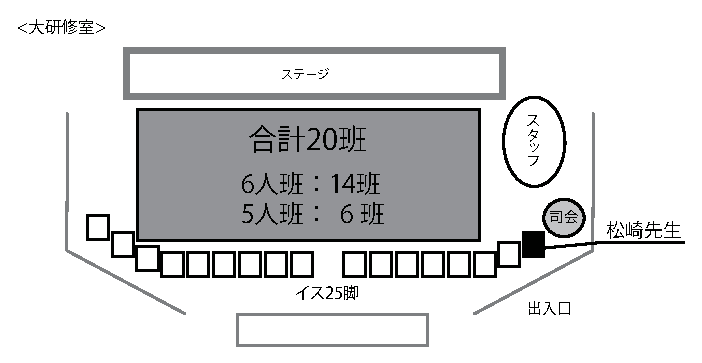
\includegraphics[scale=1.5]{./08/nyushoshiki.eps}
  \caption{入所式配置図}
  \label{nyusyosiki}
  \end{center}
\end{figure}


\subsection{必要物品}
\begin{itemize}
\item マイク:2つ(幡多)
\item マスキングテープ:1個
\item 教職員の座席用紙
\item 野外炊事班のプラカード:20個(名簿入り:誘導用)
%\item 靴を入れていた袋を回収する用のビニール袋:3つ
\end{itemize}

\clearpage

\subsection{各班代表者}
\begin{table}[htb]
  \begin{center}
  \begin{tabular}{|l|l||l|l||l|l||l|l||l|l|} \hline
  1班 & 生野 & 2班 & 塩谷 & 3班 & 伊崎 & 4班 & 北村 & 5班 & 丸田 \\ \hline
  6班 & 吉田 & 7班 & 青山 & 8班 & 別役 & 9班 & 新田 & 10班 & 高橋(龍) \\  \hline
  11班 & 横田 & 12班 & 渡辺 & 13班 & 角原 & 14班 & 小松 & 15班 & 石野 \\ \hline
  16班 & 江川 & 17班 & 中島 & 18班 & 高島 & 19班 & 東 & 20班 & 新川 \\ \hline
    \end{tabular}
  \end{center}
\end{table}


\subsection{備考}
\begin{itemize}
\item 先遣隊,後遣隊や荷卸により班代表が揃ってない場合は,前後の班代表が整列を行う
%\item 下出は入所式開始に間に合わないため,尾辻は17班の整列を行う
\item 整列時,新入生と教職員は対面した状態で整列させる
\item 司会者は,新入生へ入所式開始前に椅子を前に並ぶことを促す
\item 大研修室のキャパシティがギリギリであるため,司会と班代表が詰めて座るように促す
\item 教員紹介の後,新入生は反対側を向いて施設職員さんのお話を聞く
\item 時間の関係上,速やかに行動できるように各々がやるべきことを把握しておく
\item 最初に話す松崎先生は施設職員に向けたあいさつがある
\item 教員紹介は1人あたり1分程度にする
\item 教員紹介に来られなかった教員は司会が紹介を行う
\end{itemize}


 %\subsection{連絡事項}
% ◯◯は教員紹介終了後,報告LINEに野外炊事場に向かうことを伝える

%\include{end}
